\section{error\_\-in\_\-lx Class Reference}
\label{classerror__in__lx}\index{error_in_lx@{error\_\-in\_\-lx}}
Inheritance diagram for error\_\-in\_\-lx::\begin{figure}[H]
\begin{center}
\leavevmode
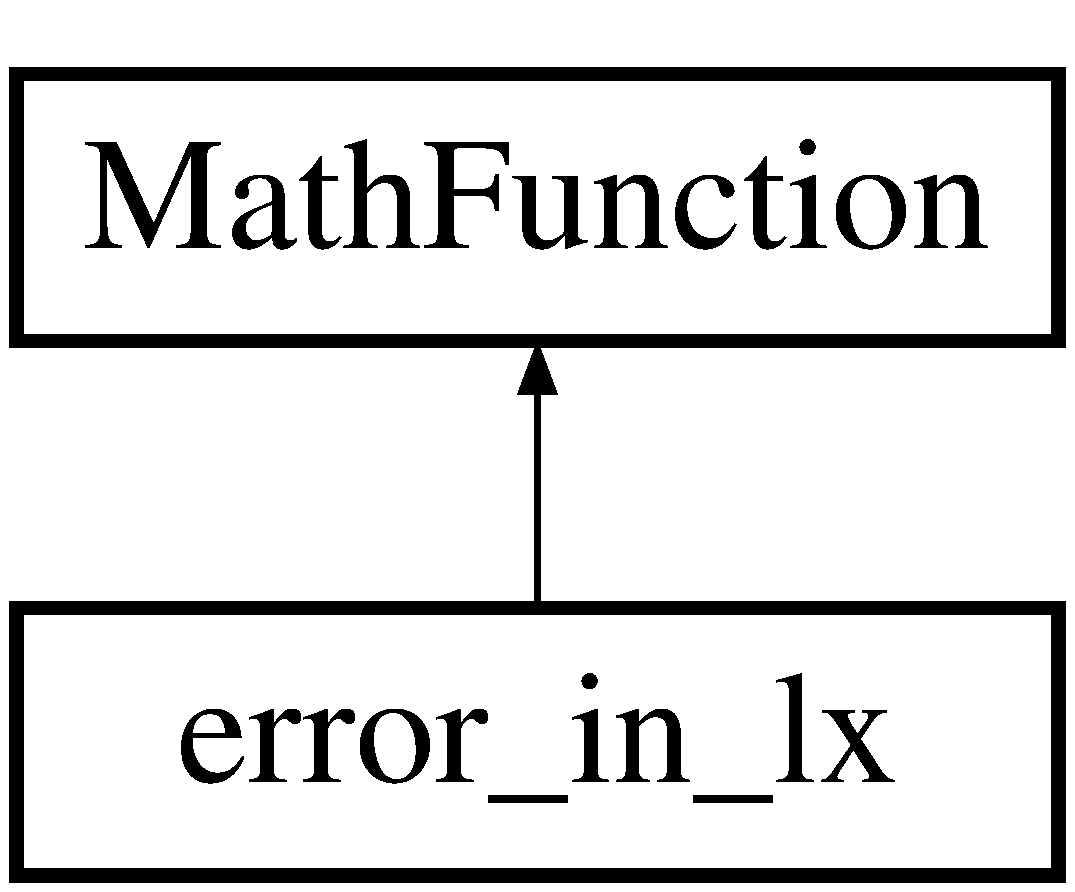
\includegraphics[height=2cm]{classerror__in__lx}
\end{center}
\end{figure}
\subsection*{Public Member Functions}
\begin{CompactItemize}
\item 
\bf{error\_\-in\_\-lx} (\bf{Double\_\-2D} const \&measured\_\-intensity, \bf{Double\_\-2D} const \&estimated\_\-intensity, double ly)\label{classerror__in__lx_6e6d4ebfe39fdc2634da8d7c4b040f47}

\item 
virtual double \bf{call} (double lx)\label{classerror__in__lx_45eac67d018c9562c8099ede2ff8a1a6}

\end{CompactItemize}
\subsection*{Private Attributes}
\begin{CompactItemize}
\item 
double \bf{ly\_\-}\label{classerror__in__lx_0d11d91905e3478eea1e4191ef3eba90}

\item 
\bf{Double\_\-2D} const \& \bf{estimated\_\-intensity\_\-}\label{classerror__in__lx_85bdc0e073e46d3f7497b06951747715}

\item 
\bf{Double\_\-2D} const \& \bf{measured\_\-intensity\_\-}\label{classerror__in__lx_0a61fa8b39c2c1fa63e01ab8b876d533}

\item 
std::map$<$ double, double $>$ \bf{cache}\label{classerror__in__lx_31198834676c694a170da5652c401d5d}

\end{CompactItemize}


\subsection{Detailed Description}




Definition at line 110 of file Partial\-Char\-CDI.h.

The documentation for this class was generated from the following file:\begin{CompactItemize}
\item 
Partial\-Char\-CDI.h\end{CompactItemize}
